% !TEX root =  main.tex
\section{Open-domain Event Schemas}

Event schemas specify the typical participants in an event, their roles within the schema. In this section, we describe our proposed approach for automatically constructing open-domain schemas from a large corpora. Our approach builds on our preliminary work for generating schemas. The key intuition behind our approach is that frequently co-mentioned entities and relations can be generalized to capture typical participants and their roles within the schema. Accordingly we develop a simple model for capturing co-occurring relations (Rel-grams) and a page-rank based solution for grouping relations belonging to a schema. Figure~\ref{fig:schema-generation} shows the architecture of our system. 
\begin{figure}[htbp]
\vspace{-2ex}
\begin{center}
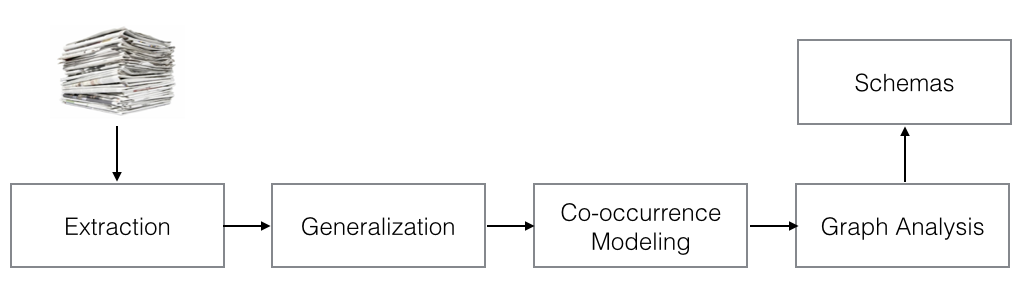
\includegraphics[height=1.75in, width=5.25in]{figures/schema-architecture}
\vspace{-4ex}
\caption{\label{fig:schema-generation}Schema Generation Pipeline}
\end{center}
\vspace{-2ex}
\end{figure}
Starting from a large collection of stories we first extract a generalized representation of the event mentions in the text. Then, we compute the co-occurrence statistics between the generalized mentions. Next, we identify relations to seed schema generation. We then construct a relation graph starting from the seed, and use graph analysis algorithms to identify the relations that belong to the schema. As a final step we resolve co-referring entities and relations and output the schema. 
There are several fundamental challenges in all stages of the pipeline. In this section, we will detail the challenges and the directions that this project will investigate for each stage.
%We use a richer representation, design techniques for generalizing arguments to an appropriate level, investigate graph-based formalisms that can effectively model sense and topic-drift issues during clustering, and build a learning-based approach for effectively scoring the generated schemas.
 
\subsection{Extraction}

The first stage in our pipeline involves extracting and representing event mentions from text. Representing information in sentences using extractions is an inherently lossy procedure. On the other hand retaining all information in a sentence doesn't scale well. Our preliminary work showed that one of the fundamental challenges in learning schemas from text is the context vs. sparsity trade-off in representation. Previous approaches used extremely limited context to represent events using (subject, verb) and (verb, object) pairs (e.g., Chambers and Jurafsky, 2009). Using such limited representations lead to incoherent schemas which mix distinct events. On the other hand, capturing more context using entire relation triples of the form (arg1, relation, arg2) leads to improved results. However, we still find that using a representation that is close to the source text has two fundamental sparsity problems: 1) Using specific mentions of events doesn't provide any generalization power. 2) Syntactic and lexical variability can mislead the system into treating the different mentions of the same event as separate events. 

To address these challenges, we propose to explore the combination of Open IE extractions with semantic role annotations. Semantic roles present a nice intermediate between ontology-free Open-IE and tight semantic ontology in closed IE systems. The thematic roles sought by SRL systems are general purpose roles that apply to a wide variety of relations. The key advantage with semantic roles is that unlike Open IE arguments, semantic role assignments are not susceptible to simple syntactic transformation and because the arguments are thematic roles, it is easy to encode N-ary relations compactly. We plan to use one of the many off-the-shelf implementations (e.g., Clear SRL~\cite{}, SemaPro~\cite{}) available\footnote{While accuracy of role labeling is important, less than perfect role labeling is not problematic in our architecture, since the roles only serve to provide a normalized argument structure -- the name of the role itself is not particularly relevant.}. 

\subsection{Generalization}

Extractions yield information about specific mentions. Generalizing from these specific mentions is the key step in extracting knowledge about types of events. This involves mapping specific instances (e.g., Barrack Obama) to an appropriate class (e.g., US President). This immediately raises two basic questions: 1) What is the underlying ontology of classes? 2) How does one map the arguments and relations to the appropriate class? For example, depending on the relation at hand {\em Barrack Obama} may map to a {\em US President}, {\em Senator}, or {\em Person}.  

{\textbf Ontology} In this work, we will leverage existing resources such as Freebase, NELL and WordNet for constructing the ontology for entities and relations. Freebase is a crowd-sourced and curated knowledge base that contains more than 43,000 types (i.e., classes)~\footnote{as of September 1st, 2014.}. Entity classification systems~\cite{xiao}, entity linking systems~\cite{tlin}, and relation extraction systems~\cite{multir} have been developed to identify instances of Freebase types. These provide a great starting 
point for mapping named entities and some subset of relations into Freebase. Events also involve common noun arguments (e.g, The fire burned down {\em the entire condominium} in 2 hours.). It is important to be able to generalize {\em condominiums} to its class {\em building}. We use Wordnet type hierarchy to assign classes to common nouns.

The ontologies, as the name implies, are hierarchies of classes. Determining what an appropriate level of generalization is a tricky problem. In our preliminary work we created multiple entires one for each type in the hierarchy up to the root. In addition to being inefficient, this method cannot be tuned to select a desired level of generalization. We propose to investigate prior work on selectional preferences and class models~\cite{} to determine the appropriate class assignment given an extraction.
 
\subsection{Co-occurrence Modeling}

This the most straight-forward piece of the pipeline, which estimates the co-occurrence probabilities of generalized event mentions. We will follow the template in our preliminary work on Rel-grams generation to produce a large table of co-occurrence frequencies and evaluate standard conditional probability estimation techniques and approaches for combining estimates obtained over different windows of document level co-occurrence. The key implementation challenge here is scaling to large collections. Rel-gram computation involves counting items that are linear in the size of the collection\footnote{With a constant proportional to the square of the average size of a document.}. We will leverage the many Map-Reduce implementation optimizations that we developed for our preliminary work.
 
\subsection{Schema Generation}

The main intuition behind schema generation is that frequently co-mentioned relations belong to the same schema and contain the salient entities and their roles. We gather frequently co-mentioned relations from the pairwise co-occurrence model. As we alluded to earlier, not all stories about an event type will mention (or necessarily) have the same set of sub-events or entities. For example, not all lawsuits will be decided in favor of the defendant and not all lawsuits will involve the filing of briefs from friends of the court, and in some cases the story itself may omit its mention. By gathering co-mentioned relations from pairwise co-occurrence models, we implicitly allow for the aggregation of information that may sometimes be missing. 

The are two main challenges in building schemas: 1) Identifying useful seeds or starting points for schemas, and 2) Effectively selecting relations to include in a schema.

\textbf{Seeding Schemas} The pairwise co-occurrences represent a large graph where the generalized relations are nodes and co-occurrences specify edge weights. In this setting, a direct approach to gathering co-mentioned relations is to perform clustering over this graph (either bottom-up or top-down). Instead we propose to investigate a seed-based expansion approach, which has several key benefits: a) Avoids the problem of large clusters resulting from hub nodes that are general purpose relations (e.g., {\em father of}, {\em spokesperson for}). b) Allows local structure around nodes to govern the inclusion in schema, which makes it easier to design selection algorithms.  c) Allows for an on-demand clustering of graph given any starting point. As we will point out later this flexibility is desirable for both development purposes (control for the seeds), as well as for use in applications which can provide an effective circumscription of the graph based on their input.

We propose to explore a probabilistic generative model for seed selection. Given a co-occurrence model with appropriate probabilistic semantics, we can directly construct a generative probabilistic model, which specifies the probability of observing other relations having observed a specific relation. The quality of a seed can be approximated by the quality of the distribution governing its neighborhood (e.g., perplexity of observing the neighboring nodes). selecting seeds that cover diverse events, as well as providing strong anchors for building schemas. 

\textbf{Graph Analysis} 

The seed-based schema generation approach has two steps.


\subsection{Contributions}

\begin{itemize}
\item Effective representation which captures adequate context to unambiguously represent event semantics. 
\item Generalization techniques that address sparsity. 
\item Graph-based approaches that leverage graphical properties to address sense and topic-drift. 
\item Scalable method for effectively scoring generated schemas. 
\end{itemize}

